\chapter{Prehľadávanie herných stromov}


\tikzset{
  cross/.style={orange, scale line widths, line width=0.9ex},
  nought/.style={teal, scale line widths, line width=0.9ex},
    value/.style={magenta, font={\fontsize{0.5cm}{0pt}\selectfont\bfseries}  }
}

    \def\sh{0.2}
    \def\tttscale{0.17}
    \def\cross(#1,#2){
      \draw[cross](#1+\sh,3-#2-\sh)--(#1+1-\sh,2-#2+\sh);
      \draw[cross] (#1+\sh,2-#2+\sh)--(#1+1-\sh,3-#2-\sh);}
    \def\nought(#1,#2){\draw[nought](#1+0.5,2.5-#2) circle (0.3);}
\def\tttgrid#1{
      \filldraw[yellow!8!white](0,0) rectangle (3,3);
      \draw(0,0) grid (3,3);
        \gdef\tmp{#1} 
        \gdef\w{0}
        \foreach\y in {0,1,2} {
          \foreach\x in {0,1,2} {
              \isnextbyte[q]{X}{\tmp}
              \if T\theresult\cross(\x,\y)\xdef\w{1}\xdef\fx{\x}\xdef\fy{\y}\fi
              
              \isnextbyte[q]{Y}{\tmp}
              \if T\theresult\cross(\x,\y)\xdef\w{1}\xdef\tx{\x}\xdef\ty{\y}\fi
              
              \isnextbyte[q]{x}{\tmp}
              \if T\theresult\cross(\x,\y)\fi
              
              \isnextbyte[q]{O}{\tmp}
              \if T\theresult\nought(\x,\y)\xdef\w{2}\xdef\fx{\x}\xdef\fy{\y}\fi
              
              \isnextbyte[q]{Q}{\tmp}
              \if T\theresult\nought(\x,\y)\xdef\w{2}\xdef\tx{\x}\xdef\ty{\y}\fi
              
              \isnextbyte[q]{o}{\tmp}
              \if T\theresult\nought(\x,\y)\fi
              \gobblechar{\tmp}
              \xdef\tmp{\thestring}
            } 
        }
        \if\w1\draw[orange,thick](\fx+0.5,2.5-\fy) -- (\tx+0.5,2.5-\ty);\fi
        \if\w2\draw[teal,thick](\fx+0.5,2.5-\fy) -- (\tx+0.5,2.5-\ty);\fi
}

    \def\tttinl#1{
      \begin{tikzpicture}[scale=0.23,baseline=0.8mm]\tttgrid{#1}\end{tikzpicture}
    }
    \def\crossinl{
      \begin{tikzpicture}[scale=0.45,baseline=1.2mm]\cross(0,2)\end{tikzpicture}
    }
    \def\noughtinl{
      \begin{tikzpicture}[scale=0.45,baseline=1.2mm]\nought(0,2)\end{tikzpicture}
    }

    \def\ttt(#1)#2{
      \begin{scope}[shift={(#1)}]\begin{scope}[scale=\tttscale]\begin{scope}[shift={(-1.5,-1.5)}] 
      \tttgrid{#2}
      \end{scope}\end{scope}\end{scope}
    }
    %1->2 1->3 4krat
    \def\prt#1#2#3#4{
    \foreach\x in {0,...,#4} {
      \pgfmathsetmacro{\tmp}{\x/#4}
      \coordinate (ptmp) at ($(p#2)!\tmp!(p#3)$);
      \draw[teal,dotted] (p#1)--(ptmp) ;
      \draw[teal] (p#1) -- ($(p#1)!0.6!(ptmp)$);
    }
    }
    
    \def\vals<#1>#2#3{
%    \only<#1>{
    \foreach \p/\v in {#2} {
      \node[value,black] at ($(p\p)+(0.015,-0.015)$) {\v};
      \node[value,#3] at (p\p) {\v};
%     }
    }
   }



Cieľom tejto časti je naprogramovať hráča, ktorý by hral \btr. 
Začneme skromne:



\begin{uloha}
  \label{uloha:randomplayer}
  Pokračuj v projekte z úlohy~\ref{uloha:btr1}. Do súborov \vb{board.h}/\vb{board.cc} pridaj
  načítanie ťahu zo vstupu (načíta sa reťazec napr. \vb{``c5-d6''}). 

\begin{lstlisting}
std::istream& operator>> (std::istream &, Move &);
\end{lstlisting}

  Pridaj rovnaké načítanie aj pre \vb{Square} a \vb{Board} (to môže byť zoznam políčok bieleho
  a zoznam políčok čierneho, oba ukončené bodkočiarkou a nasledované číslom
  polťahu, napr \vb{``a3 b4; c7 d8; 12''}).
  Vyrob triedu \vb{RandomPlayer} s metódou 

\begin{lstlisting}
Move findMove(const Board& b)
\end{lstlisting}

  ktorá vráti náhodný prípustný ťah.
  Napokon uprav \vb{main.cc} tak, aby hral hru: načíta ťah bieleho, skontroluje, či je korektný,
  vypíše šachovnicu, spraví náhodný ťah čierneho, \ldots\ až kým niekto nevyhrá.
\end{uloha}

Toto nebolo ťažké, ale zjavne to má 
od dôstojného protivníka ďaleko.
Ak chceme naprogramovať lepšieho hráča, je dobré si najprv preskúmať, čo vlastne chceme. To, čo si budeme hovoriť, platí nielen pre \btr, ale všeobecne pre hry dvoch hráčov (ktorí sa striedajú na ťahoch),
sú {\em s úplnou informáciou} 
(t.j. obaja hráči vidia všetko, na rozdiel napr. od väčšiny kartových hier),\indexItem{Alg}{zero-sum hry, stratégia} 
sú {\em deterministické} (t.j. nehrá pri nich úlohu náhoda, ako napr. pri hre Monopoly), 
a sú {\em s nulovým súčtom} ( {\em zero-sum}
t.j. výhra jedného hráča je prehrou druhého). V takýchto hrách budeme hľadať 
stratégiu pre jedného hráča. Čo je to stratégia? Niečo, čo mi v každej situácii povie, ako mám hrať.
Zoberme si napr. Tic-Tac-Toe. Ako by mohla vyzerať stratégia pre hráča \hbox{\crossinl?}
Začne napr. tým, že stratégia mu povie dať prvý ťah do stredu. Teraz je na ťahu \noughtinl a \crossinl musí byť
pripravený odpovedať na všetky možné ťahy \noughtinl. 
V skutočnosti sú iba dva, ostatné možnosti sú symetrické.\\


\centerline{
  \begin{tikzpicture}[scale=1.52]

    \foreach\y in {4,2,0}
    \filldraw[orange!10!white] (-1.5,\y+0.5) rectangle (7.5,\y+1.5);
    \foreach\y in {5,3,1,-1}
    \filldraw[teal!10!white] (-1.5,\y+0.5) rectangle (7.5,\y+1.5);


    \foreach\x/\y[count=\n] in {
      3/6,1/5,5/5,1/4,5/4,  % p1 .. p5
      0/3, 2/3, 3/3, 4/3, 5/3, 7/3,  % p6 ... p11
                3/2, 4/2, 5/2, 7/2,  % p12 ... p15
      2.5/1, 3.5/1, 4.5/1, 5.5/1, 
      2.5/0, 3.5/0, 4.5/0, 5.5/0,
      0/2, -1/1, 1/1, 1/1, -1/0, % p24 .. p28
      -1.5/-0.71,-0.5/-0.71,
      2/2 % p31 - afterthought
    }
    \coordinate(p\n)at(\x,\y);

%    \only<3>{
%      \draw[yellow!30, line width=2.8ex] (p1)--(p2)--(p4)--(p6)--(p24)--(p25)--(p28)--(p30) (p28)--(p29);
%    }
    \draw[teal](p1)--(p2) (p1)--(p3) (p4)--(p6) (p4)--(p7) (p5)--(p8) (p5)--(p9) (p5)--(p10) (p5)--(p11)
    (p13)--(p16) (p13)--(p17) (p13)--(p18) (p13)--(p19)
    (p24)--(p25) 
    ;
    \prt4675    
    \prt5{10}{11}3
    \prt{24}{25}{27}3

    \draw[teal,dotted] (p28)--(p29) (p28)--(p30);

    \draw[orange,snake=coil,segment aspect=0, segment amplitude=1pt, segment length=2pt, line after snake=0pt] (p2)--(p4) (p3)--(p5)
    (p6) -- (p24) (p25)--(p28) (p7) -- (p31)
    (p8)--(p12) (p9)--(p13) (p10)--(p14) (p11)--(p15)
    (p16)--(p20) (p17)--(p21) (p18)--(p22) (p19)--(p23)
    ;
    \ttt(p1){....x....}
    \ttt(p2){o...x....}
    \ttt(p3){.o..x....}
    \ttt(p4){o..xx....}
    \ttt(p5){.o..x.x..}
    \ttt(p6){o..xxo...}
    \ttt(p7){o..xx...o}
    \ttt(p31){o..XxY..o}
    \ttt(p8){oo..x.x..}
    \ttt(p9){.oo.x.x..}
    \ttt(p10){.o.ox.x..}
    \ttt(p11){.o..x.x.o}
    \ttt(p12){ooY.x.X..}
    \ttt(p13){xoo.x.x..}
    \ttt(p14){.oYox.X..}
    \ttt(p15){.oY.x.X.o}
    \ttt(p16){xooox.x..}
    \ttt(p17){xoo.xox..}
    \ttt(p18){xoo.x.xo.}
    \ttt(p19){xoo.x.x.o}
    \ttt(p20){Xooox.x.Y}
    \ttt(p21){Xooox.x.Y}
    \ttt(p22){Xooox.x.Y}
    \ttt(p23){Xooxx.Y.o}

    \ttt(p24){o.xxxo...}
    \ttt(p25){o.xxxoo..}
    \ttt(p28){o.xxxoox.}
%    \vals<2-3>{3/1}{teal}
%    \vals<3>{1/0}{teal}
  \end{tikzpicture}}

Ak \noughtinl zahrá \tttinl{.o..x....}, stratégia povie \crossinl zahrať \tttinl{.o..x.x..}
a ak \noughtinl zahrá \tttinl{o...x....}, tak mu povie zahrať \tttinl{o..xx....} atď.
Stratégia pre \crossinl je teda strom, v ktorom vo vrcholoch sú herné pozície, pričom 
ak je na ťahu \crossinl, vyberie sa jeden ťah a ak je na ťahu \noughtinl, musia sa brať
do úvahy všetky ťahy. Pozri sa teraz, čo sa stane, ak sa vyskytne pozícia \tttinl{.o..x.x..}
(na ťahu je \noughtinl). Nech \noughtinl zahrá hocičo, \crossinl môže vyhrať buď v nasledujúcom ťahu,
alebo (ak \noughtinl zahrá \tttinl{.oo.x.x..} a následne \crossinl zahrá \tttinl{xoo.x.x..})
v druhom ťahu. Pozíciu, z ktorej pre \crossinl existuje vyhrávajúca stratégia (t.j. má zaručenú
výhru nech \noughtinl hrá hocijako) voláme vyhrávajúca (a dávame jej hodnotu 1). 
Podobne, ak existuje vyhrávajúca stratégia pre \noughtinl (t.j. \noughtinl vie vyhrať,
nech \crossinl robí čokoľvek), takúto pozíciu 
voláme prehrávajúca (pozeráme sa na svet z pohľadu \crossinl) a
dávame jej hodnotu -1. V našom prípade sme videli, že \tttinl{.o..x.x..} je vyhrávajúca pozícia,
a preto aj \tttinl{.o..x....} je vyhrávajúca (\crossinl je na ťahu a môže zahrať
\tttinl{.o..x.x..}). Takže od \noughtinl
je chyba zahrať na začiatku \tttinl{.o..x....}.


Pozrime sa teraz na pozíciu \tttinl{o...x....}. Stratégia pre \crossinl (ktorú som celú 
nedokreslil, ale je ľahké si ju domyslieť) mu zaručí, že nech \noughtinl robí čokoľvek, 
\crossinl nikdy neprehrá. Takže \crossinl má {\em neprehrávajúcu} stratégiu. Môže
mať inú stratégiu, ktorá by bola vyhrávajúca?

\def\ulohaTarget{None}
\begin{uloha}
  Nájdi neprehrávajúcu stratégiu pre \noughtinl z pozície \tttinl{o...x....} 
  (na ťahu je \crossinl).
\end{uloha}
\def\ulohaTarget{Dir}


Čo to pre hráča \crossinl znamená, že \noughtinl má neprehrávajúcu stratégiu?
\crossinl vie, že ak by sa odchýlil od svojej neprehrávajúcej stratégie, \noughtinl 
ho určite nenechá vyhrať, a navyše sa mu môže ešte stať, že prehrá. Preto je preňho lepšie
držať sa svojej neprehrávajúcej stratégie. A rovnako pre \noughtinl. \tttinl{0...x....}
je príkladom pozície, ktorej hovoríme {\em remízová} a dávame jej hodnotu 0. Je to pozícia,
v ktorej obaja hráči majú neprehrávajúcu stratégiu -- optimálne hra vždy vedie k remíze.
Môžu byť aj iné pozície ako vyhrávajúca, prehrávajúca a remízová? 
Zjavne nie. Predstav si totiž kompletný strom hry. Každý koncový vrchol má hodnotu $0$, $1$, alebo $-1$,
lebo na konci hry buď niekto vyhrá, alebo je remíza. Teraz sa pozrime na také vrcholy, 
ktoré vedú len do koncových vrcholov. Ak je v takomto vrchole $V$ na ťahu \crossinl a existuje
ťah, v ktorom by vyhral (teda ťah do vrchola s hodnotou 1), \crossinl urobí ten ťah a vyhrá.
Hodnota $V$ je preto 1. Ak ťah, ktorý by \crossinl zaručil výhru neexistuje, ale existuje
ťah do remízy, \crossinl môže urobiť ten a hodnota $V$ bude 0. V opačnom prípade (t.j. nech \crossinl
urobí čokoľvek, tak prehrá) bude hodnota $V$ $-1$. Inými slovami, ak je vo $V$ na ťahu \crossinl,
hodnota $V$ bude maximum hodnôt všetkých jeho synov. Podobne ak je vo vrchole $V$ na ťahu \noughtinl,
hodnota $V$ je minimum hodnôt jeho synov. Takto môžeme postupovať ďalej: vždy zoberieme vrchol $V$,
ktorého všetci nasledovníci majú priradenú hodnotu (rozmysli si, že taký vrchol vždy musí existovať) 
a priradíme hodnotu aj $V$. 

 
Týmto sme sa presvedčili, že pre akúkoľvek (deterministickú, s úplnou informáciou, s nulovým súčtom) \indexItem{Alg}{MiniMax a NegaMax}
hru je každá pozícia vyhrávajúca, prehrávajúca, alebo remízová. To nielenže znamená, 
že vždy existuje optimálna
stratégia, ale v predchádzajúcom odstavci sme aj opísali postup (nazývaný {\scshape MiniMax}), ako
ju nájsť. Tento postup vieme naprogramovať jednoduchou rekurzívnou procedúrou \prg!int value(const Board &b)!:
ak je to koncová pozícia, vrátime víťaza, inak vyrobíme všetky možné ťahy, rekurzívne zistíme ich hodnoty a
vrátime minimum alebo maximum, podľa toho, ktorý hráč je na ťahu.

Aby sme nemuseli
zvlášť riešiť maximalizujúceho hráča (volajme ho biely, \crossinl, alebo {\scshape Max}) a minimalizujúceho
hráča (čierny, \noughtinl, {\scshape Min}), je pri implementácii príjemnejšie vracať hodnotu pozície z pohľadu hráča, 
ktorý je 
práve na ťahu (t.j. hodnota 1 znamená vyhrávajúca pozícia pre hráča, ktorý je práve na ťahu). 
V tomto pohľade každý hráč hľadá ťah, ktorý maximalizuje hodnotu pozície. 
Pri tom sa dá využiť vlastnosť nulového súčtu: čo je výhra (1) z pozície bieleho, je prehra
(-1) z pozície čierneho. Keď rekurzívne zistím hodnoty nasledovníkov, dostanem ich z pozície súpera, takže 
z môjho pohľadu budú čísla opačné. Tento spôsob programovania sa zvykne volať {\scshape NegaMax}.
Ak si do triedy \vb{Board} dorobím metódu \prg!int Board::toPlay() const;!
ktorá vráti $1$, ak je na ťahu biely a $-1$ ak je na ťahu čierny, môžem napísať:

\vbox{
\begin{lstlisting}
// hodnota pozície b
int value(const Board &b) {
  int side = b.toPlay();  // 1, -1 podľa toho, kto je na ťahu
  int w = b.winner();     // má b víťaza?
  if (w == White) return side;  // ak vyhral biely a je práve na ťahu, tak 1, 
                                // ak vyhral biely a na ťahu je čierny, tak -1
  if (w == Black) return -side; // ak vyhral čierny, tak podobne

  auto ms = b.legalMoves();  // vyrobím všetky prípustné ťahy
  int mx = -1;               // hodnota z pohľadu toho, kto je na ťahu

  for (int i = 0; i < ms.size(); i++) { // ideme testovať každý možný ťah
    Board bb = b;
    bb += ms[i];         // urob daný ťah
    int v = -value(bb);  // rekurzívne vyrátaj hodnotu nasledovníka
                         // výsledok je z pohľadu protivníka, 
                         // takže z môjho pohľadu je opačný
    if (v > mx) mx = v;  // pamätám si doteraz najlepšiu možnosť
    if (mx == 1) break;  // lepšie už nemôže byť, netreba pokračovať
  }
  return mx; 
}
\end{lstlisting}
}

\begin{uloha}
  Napíš program, ktorý prečíta zo vstupu pozíciu, nájde jej hodnotu (1 alebo -1 z pohľadu bieleho) a vypíše ju. Potom vypíše všetky prípustné ťahy 
  a hodnoty pozícií, do ktorých vedú. Používateľ potom môže zadať niektorý ťah a opäť sa nájde hodnota pozície a všetkých prípustných ťahov.
\end{uloha}

\begin{outputBox}
c6 d5 h6; d6 b3 g7 h8; 0
    a   b   c   d   e   f   g   h
  +---+---+---+---+---+---+---+---+
8 |   |   |   |   |   |   |   | O | 8
  +---+---+---+---+---+---+---+---+
7 |   |   |   |   |   |   | O |   | 7
  +---+---+---+---+---+---+---+---+
6 |   |   | X | O |   |   |   | X | 6
  +---+---+---+---+---+---+---+---+
5 |   |   |   | X |   |   |   |   | 5
  +---+---+---+---+---+---+---+---+
4 |   |   |   |   |   |   |   |   | 4
  +---+---+---+---+---+---+---+---+
3 |   | O |   |   |   |   |   |   | 3
  +---+---+---+---+---+---+---+---+
2 |   |   |   |   |   |   |   |   | 2
  +---+---+---+---+---+---+---+---+
1 |   |   |   |   |   |   |   |   | 1
  +---+---+---+---+---+---+---+---+
    a   b   c   d   e   f   g   h
1
c6-b7: 1
c6-c7: 1
c6-d7: 1
d5-e6: -1
h6-g7: 1
h6-h7: 1
\end{outputBox}


Problém s týmto programom je v tom, že na to, aby našiel hodnotu nejakej pozície, musí prehľadať celý jej podstrom. Pre pozície, ako tá na predchádzajúcom príklade, to je dostatočne málo,
ale koľko by to bolo, keby si zadal štartovaciu pozíciu? Ťažko to povedať presne, ale keby sme veľmi zhruba odhadli, že v priemere má pozícia 12 prípustných ťahov (je 16 kameňov,
takže najviac môže byť 48 možných ťahov, ale väčšinou je to menej) a partia trvá 30 ťahov (t.j. 60 polťahov), tak strom by mal 
$$12^{60}=56347514353166785389812313795980500551139163800306781874894667776$$
vrcholov. Toľko čakať určite nechceš.



Keď chceme použiť {\scshape MiniMax} na praktické hranie, najjednoduchší spôsob je
obmedziť hĺbku stromu.  Namiesto toho, aby sme pre danú pozíciu prehľadávali
celý podstrom až po koncové pozície, pôjdeme iba do fixnej hĺbky (napr. štyri
ťahy dopredu) a potom odhadneme, do ako dobrej pozície sme sa dostali. Na to
budeme potrebovať nejakú funkciu \vb{eval}, ktorá zoberie pozíciu a vráti odhad
jej hodnoty: číslo z rozsahu $[-1,1]$.  Môžeš sa spýtať, prečo teda, ak budeme
mať takú vyhodnocovaciu funkicu, ju nepoužijeme priamo, ale strácame čas 
prehľadávaním. Problém je v tom, že vyrobiť takú funkciu vôbec nie je ľahké a
funkcia, ktorú budeme mať, bude nutne nepresná. A dúfame, že prehľadávanie nám
pomôže: predpokladáme, že aj taký zlý ťah, ktorý by naša funkcia neodhalila,  sa po pár ťahoch prejaví tak, že aj
jednoduchá funkcia (napr. taká, ktorá len počíta počet kameňov) to zistí.

\begin{uloha}
  Naprogramuj hráča \vb{MinimaxPlayer}. Podobne ako \vb{RandomPlayer} z úlohy \ref{uloha:randomplayer} bude mať metódu 
  \prg!Move findMove(const Board& b)!. V tej sa pre každý prípustný ťah nájde hodnota výslednej pozície pomocou  prehľadávania 
  podobne ako vo funkcii \vb{value}, ale navyše s parametrom \vb{hlbka}, ktorý sa v každom rekurzívnom
  volaní bude zmenšovať. Keď dosiahne nulu, zavolá sa metóda \prg!MinimaxPlayer::eval(const Board&)!. 
  Môžeš zatiaľ použiť niečo veľmi jednoduché, napr. 

  \begin{lstlisting}
  (pocet_kamenov_bieleho - pocet_kamenov_cierneho)/16.0
  \end{lstlisting}
  
  (to delenie \vb{16.0} je tam preto, aby som dostal číslo z intervalu $[-1,1]$, ale vlastne to ani nepotrebujem). Výsledkom volania \vb{findMove} bude ten ťah, ktorý sa
  dostane do najlepšej pozície (ak je takých viacero, tak vyber náhodný).  Podobne ako v úlohe \ref{uloha:randomplayer} sprav, aby
  \vb{MinimaxPlayer} hral hru. 
\end{uloha}


Čím väčšiu hĺbku prehľadávania zvolím, tým dlhšie trvá urobiť ťah. Pri hĺbke 4
to u mňa išlo ešte celkom rýchlo (zhruba 1-2s na ťah), pri hĺbke 5 to už ale bolo aj
okolo 2min na ťah.  A síce hrá oveľa lepšie, ako náhodný hráč, stále to ani s
hĺbkou 5 nie je nič moc. Je ale veľa spôsobov, ako sa to dá zlepšiť. 

%%%%%%%%%%%%%%%%%%%%%%%%%%%%%%%%%%%%%%%%%%%%%%%%%%%%%%%%%%%%%%%%%
\section*{$\alpha\beta$-orezávanie}\indexItem{Alg}{orezávanie herných stromov}
           
           \def\Biglist{
            1.5/{2,4,2,2,3,2,2,2,3,2,3,2,2,4,3,2,3,3,2,2,3,2,3,2}, 
            3/{2,2,2,2,2,3,5,2,2,2}, 
            4/{3,5,2},
            5/{3}}
\def\crossnode(#1){\begin{scope}[shift={(#1)}]\filldraw[fill=white](-0.5,-0.5)rectangle(0.5,0.5);\begin{scope}[shift={(-0.5,-0.5)}]\cross(0,2)\end{scope}\end{scope}}
\def\noughtnode(#1){\begin{scope}[shift={(#1)}]\filldraw[fill=white](-0.5,-0.5)rectangle(0.5,0.5);\begin{scope}[shift={(-0.5,-0.5)}]\nought(0,2)\end{scope}\end{scope}}

       \def\coords{
          \foreach \v in {1,...,60 } 
            \coordinate(p0x\v) at (\v,0);
          \foreach \h/\list[count=\lev] in \Biglist{
           \gdef\l{1}
           \foreach \d[count = \cnt] in \list {
             \pgfmathtruncatemacro{\r}{\l+\d-1}
             \pgfmathtruncatemacro{\prevlev}{\lev-1}
             \coordinate(p\lev x\cnt) at ($(p\prevlev x\l)!0.5!(p\prevlev x\r) + (0,\h)$);
             \pgfmathtruncatemacro{\r}{\r+1}
             \xdef\l{\r}
           }
         }
       }

       \def\base[#1]{
          \gdef\y{0}
          \foreach\h in {1.5, 3, 4, 5} {
            \pgfmathsetmacro{\tmp}{\y+\h}
            \xdef\y{\tmp}
            \draw[gray!60,dotted](1,\y) -- (60,\y);
          }
          \foreach \h/\list[count=\lev] in \Biglist{
           \gdef\l{1}
           \foreach \d[count = \cnt] in \list {
             \pgfmathtruncatemacro{\r}{\l+\d-1}
             \pgfmathtruncatemacro{\prevlev}{\lev-1}
             \filldraw[#1](p\lev x\cnt) circle (0.1);
             \foreach \i in {1,...,\d} {
               \pgfmathtruncatemacro{\tmp}{\l+\i-1}
               \draw[#1] (p\lev x\cnt) -- (p\prevlev x\tmp);
             }
             \pgfmathtruncatemacro{\r}{\r+1}
             \xdef\l{\r}
           }
         }
       }

       \def\labels{
          \foreach \r/\n in {1/24,3/3} {
             \foreach \i in {1,...,\n} {
                \noughtnode(p\r x\i)
             }
          }
          \foreach \r/\n in {2/10,4/1} {
             \foreach \i in {1,...,\n} {
                \crossnode(p\r x\i)
             }
          }
       }



Prvý spôsob, ako vylepšiť {\scshape MiniMax}, je založený na  zistení, že dosť často sa veľa vrcholov
prehľadáva zbytočne. Ak sa na  {\scshape MiniMax} pozrieme pohľadom zdola-hore, máme listy, ktoré
majú hodnoty a vnútorné vrcholy, ktoré vždy vyberú niektorého (najväčšieho alebo najmenšieho)
syna. Celé prehľadávanie si preto môžeme prestaviť tak, že jednotlivé hodnoty sa presúvajú z 
listov smerom hore

  
      \centerline{
        \begin{tikzpicture}[scale=0.25]
          \def\stripe[#1]#2#3{
            \foreach \d[count=\i] in {#3} {
              \if\i1
                  \xdef\last{p0x\d}
                  \node[below] at (\last) {\scriptsize$#2$};
              \else
                  \pgfmathtruncatemacro{\tmp}{\i-1}
                  \draw[#1,line width=1.5mm] (\last) -- (p\tmp x\d);
                  \xdef\last{p\tmp x\d}
              \fi 
            }

          }
          \coords
          %\foreach \i in {1,3,5,6,8,10,12,13,15,16,18,20,22,23,25,27,29,30,32,33,35,37,38,40,41,42,44,46,48,49,51,52,54,56,57,59} 
          %\node[below] at (p0x\i) {\scriptsize $9$};

          \def\di{teal!20}
          \def\dii{orange!30}
          \def\diii{blue!20}
          \def\div{red!20}

          \stripe[\di]{1}{2,1}
          \stripe[\dii]{7}{4,2,1}
          \stripe[\di]{3}{7,3}
          \stripe[\diii]{4}{9,4,2,1}
          \stripe[\dii]{8}{11,5,3}
          \stripe[\di]{1}{14,6}
          
          \stripe[\di]{6}{17,7}
          \stripe[\dii]{9}{19,8,4}
          \stripe[\div]{6}{21,9,5,2,1}
          \stripe[\di]{3}{24,10}
          \stripe[\dii]{7}{26,11,6}
          \stripe[\di]{5}{28,12}
          \stripe[\di]{6}{31,13}

          \stripe[\di]{1}{34,14}
          \stripe[\di]{7}{36,15}
          \stripe[\di]{5}{39,16}
          \stripe[\di]{4}{43,17}
          \stripe[\dii]{8}{45,18,7}
          
          \stripe[\dii]{9}{47,19,8}
          \stripe[\di]{2}{50,20}
          
          \stripe[\dii]{6}{53,21,9}
          \stripe[\di]{1}{55,22}
          \stripe[\diii]{5}{58,23,10,3}
          \stripe[\di]{3}{60,24}
          
          \base[black]
          \foreach \v in {1,...,60 } 
            \filldraw (p0x\v) circle (0.1);
          \labels

          \foreach \w/\p/\v in {above/4x1/6,above/3x1/4,above right/3x2/6,above/3x3/5,
          above left/2x1/7, above left/2x2/4, above/2x3/8, above/2x4/9, left/2x5/6,
          right/2x6/7, above/2x7/8, above/2x8/9, above/2x9/6, above right/2x10/5
          }{
          \node[\w = 1.5mm ] at (p\p) {\scriptsize $\v$};
        }
        \end{tikzpicture}
    }

 
Cieľom pri prehľadávaní je nájsť ten list, ktorého hodnota sa dostane až úplne hore. 
Predpokladajme teraz, že hľadáme hodnotu vrchola $v_1$, ktorý je maximalizačný. Zistili sme, 
že prvý syn má hodnotu $4$ a pokračovali sme hľadať hodnotu $v_2$.
Tam sme našli synov s hodnotami $9$, $6$, a $7$ a opäť rekurzívne hľadáme hodnotu
$v_3$. O tom sme zistili, že má synov s hodnotami $1$ a $7$. Čo teraz vieme povedať?
Nech by zvyšní synovia $v_3$ mali akékoľvek hodnoty, hodnota $v_3$ bude aspoň $7$.
Zároveň vidíme, že hodnota $v_2$ bude najviac $6$. V tomto momente preto môžeme prestať
vyhodnocovať synov $v_3$, lebo určite sa nikto z nich nedostane nad $v_2$.

  
      \centerline{
        \begin{tikzpicture}[scale=0.25]
          \coords

          \base[black!20]

          \draw (p4x1)--(p3x1) (p4x1)--(p3x2) (p3x2)--(p2x4) (p3x2)--(p2x5) 
          (p3x2)--(p2x6) (p3x2)--(p2x7)
          (p2x7) -- (p1x14) (p2x7)--(p1x15) (p2x7)--(p1x16);

          \filldraw (p3x1) circle (0.2) node[above=1.5mm] {$4$};
          \filldraw (p2x4) circle (0.2) node[above=1.5mm] {$9$};
          \filldraw (p2x5) circle (0.2) node[left=1.5mm] {$6$};
          \filldraw (p2x6) circle (0.2) node[right=1.5mm] {$7$};
          \filldraw (p1x14) circle (0.2) node[above=1.5mm] {$1$};
          \filldraw (p1x15) circle (0.2) node[left=1.5mm] {$7$};

          \crossnode(p4x1)
          \node[above=1.5mm] at (p4x1) {$v_1$};

          \noughtnode(p3x2);
          \node[above right=1.5mm] at (p3x2) {$v_2$};
          
          \crossnode(p2x7);
          \node[above=1.5mm] at (p2x7) {$v_3$};

          \foreach \v in {1,...,60 } 
            \filldraw[black!20] (p0x\v) circle (0.1);

        \end{tikzpicture}
    }


Toto pozorovanie vieme zovšeobecniť: ak prehľadávam nejaký vrchol a viem, že na niekde ceste
do koreňa je minimalizačný vrchol s hodnotou najviac $\beta$, tak viem, že žiadna hodnota
väčšia ako $\beta$ sa do koreňa nedostane, a teda akonáhle zistím, že nejaký vrchol má hodnotu
viac ako $\beta$, nemusím ďalej prehľadávať:\\

\centerline{
\begin{tikzpicture}[scale=0.45]

  \foreach\x/\y[count=\n] in {
      0/6, 2/3, 5/0
    }
    \coordinate(p\n)at(\x,\y);
  
    \draw (p1)-- (p2) (p1) -- +(-1,-1.5) (p1) -- +(0,-1.5);
    \draw (p2) -- +(-2,-1.5)  node[anchor=north]  {$0.3$}
     (p2) -- +(-0.8,-1.5)  node[anchor=north]  {$0.1$}
     (p2) -- +(0.4,-1.5)  node[anchor=north]  {$0.4$};
    \draw ($(p2)+(1,1)$) node {val $\le 0.1$};
    \draw ($(p3)+(1,1)$) node[red] {$\beta=0.1$}; 
    \draw[dashed] (p2) -- (p3);
    \draw (p3) -- ++(-2,-1.5) node[anchor=north]  {$-0.2$}
          (p3) -- ++(0,-1.5) node[anchor=north]  {$0.6$};
    \draw (p3) -- ++(2,-1.5) node [very thick, cross out,draw=red] {} ;
    \draw[red,->,shorten <= 2ex, shorten >=2ex] (4,-5) node[red] {netreba ďalej skúšať} -- ($(p3) +(2,-1.5)$) ; 
    \crossnode(p1)
    \noughtnode(p2)
    \crossnode(p3)  
\end{tikzpicture}}


Symetrická situácia je pre minimalizačné vrcholy. Ak prehľadávam nejaký vrchol a viem, že na ceste do koreňa je 
maximalizačný vrchol s hodnotou aspoň $\alpha$, tak viem, že žiadna hodnota menšia ako $\alpha$ sa do koreňa nedostane
a môžem prestať prehľadávať. 

Naprogramoval by som to tak, že do rekurzívnej funkcie \vb{findMove} by som pridal dva parametre: \vb{alpha} a \vb{beta},
v ktorých si pamätám najväčšiu známu hodnotu v maximalizačnom vrchole a najmenšiu známu hodnotu v minimalizačnom vrchole na ceste do koreňa. 
Keď prehľadávam minimalizačný vrchol, zmenšujem hodnotu \vb{beta}, akonáhle nájdem menšieho syna. Ak som v maximalizačnom 
vrchole, zväčšujem hodnotu \vb{alpha} akonáhle nájdem väčšieho syna. Do rekurzívneho volania posielam aktualizované hodnoty
\vb{alpha} a \vb{beta}. Akonáhle zistím, že hodnota vrchola, ktorý prehľadávam, je mimo intervalu $\left\langle\alpha,\beta\right\rangle$,
prestanem s vyhodnocovaním.

Podobne ako pri pôvodnom {\scshape MiniMax} prehľadávaní, aj tu môžeme využiť vlastnosť 
nulového súčtu a spojiť obe 
vetvy do jednej.  Funkcia \vb{search} bude opäť 
vracať nie skutočnú hodnotu (t.j. $1$ ako výhra bieleho a $-1$ ako výhra čierneho), ale
hodnotu z pohľadu hráča, ktorý je práve na ťahu (t.j. $1$ vyhrá a $-1$ prehrá ten, kto je v pozícii \vb{b} na ťahu).
Dostali by sme napr. niečo takéto:

\begin{lstlisting}
float search(const Board& b, int hlbka, double alpha, double beta) {
  // tu treba otestovať, či má pozícia víťaza alebo či hĺbka dosiahla 0
  // ...
  // tu začína rekurzívna časť
  auto ms = b.legalMoves();  // vyrobíme všetky prípustné ťahy
  float best = -10;          // -10 je zarážka, skutočné hodnoty máme z rozsahu -1 .. 1
  for (int i = 0; i < ms.size(); i++) {  
    Board bb = b;
    bb += ms[i];
    // striedame minimalizáciu a maximalizáciu, preto vymeníme znamienko
    // a navyše vymeníme alfu a betu
    float v = -search(bb, hlbka - 1, -beta, -alpha);
    if (v > best) best = v;           // pamätáme si doteraz najlepšiu hodnotu
    if (best > alpha) alpha = best;   // podľa nej aktualizujeme alfu
    if (alpha >= beta) break;         // ak sme našli viac ako beta, nejdeme ďalej
  }
  return best;
}
\end{lstlisting}

\begin{uloha}
  Doprogramuj triedu \vb{AlphaBetaPlayer}.
\end{uloha}

Koľko $\alpha\beta$-orezávanie pomáha, to závisí do veľkej miery od toho, v
akom poradí prechádzame strom.  Ak vždy ako prvý vyberieme najlepší ťah,
ostatné možnosti sa orežú oveľa rýchlejšie. Preto sa zvykne pole ťahov \vb{ms}
utriediť tak, aby sa zvýšila šanca, že dobrý ťah pôjde skôr. Napr.  môžem
najprv skúšať ťahy, kde sa vyhodil kameň a pod. Na druhej strane, čas, ktorý sa
spotrebuje triedením v každom vrchole, môže narastať, ak by som na triedenie
použil príliš zložitú funkciu. Takže je to niečo, s čím sa treba pohrať a dobre
to vyladiť pre konkrétnu hru.

%%%%%%%%%%%%%%%%%%%%%%%%%%%%%%%%%%%%%%%%%%%%%%%%%%%%%%%%%%%%%%%%%
\section*{Transpozičné tabuľky}\indexItem{Alg}{transpozičné tabuľky}

V \btr a aj v iných hrách sa často vyskytuje situácia, že sa do tej istej pozície dá dostať pomocou rôznych postupností
ťahov (takéto postupnosti sa zvyknú volať {\em transpozície}): napr. zo začiatočnej pozície \vb{1.d2-d3, d7-d6, 2.e2-e3, e7-e6} aj
\vb{1.d2-e3, e7-d6, 2.e2-d3, d7-e6} prídu do pozície\\

\centerline{
%\tikzset{external/force remake}
\begin{tikzpicture}[scale=0.65]
  \boardBg
  \boardGrid
  \wPs{00,10,20,30,40,50,60,70,01,11,21,32,42,51,61,71}
  \bPs{07,17,27,37,47,57,67,77,06,16,26,35,45,56,66,76}
\end{tikzpicture}
}


V našom prehľadávaní to nijak neberieme do úvahy a každú
takúto pozíciu prehľadávame nanovo.
Podobne, ako keď sme hovorili o memoizácii v kapitole~\ref{sect:dynamika}, aj teraz je prirodzené
snažiť sa nepočítať viackrát to isté, ale si vypočítané hodnoty odkladať a dúfať, že sa ešte niekedy budú hodiť.
Urobíme si preto hešovaciu tabuľku, kde si pre každú už navštívenú pozíciu budeme pamätať jej hodnotu.

Na to, aby sme mohli použiť \vb{unordered\_map} potrebujeme, ako sme hovorili v kapitole \ref{sect:hesovanie}, špecializovať
\vb{std::Hash<Board>}. V type \vb{Board} máme uložené dve 64-bitové čísla na mapy bielych a čiernych kameňov, a ešte číslo polťahu.\indexItem{Alg}{murmur hash}
Aby sme ich dobre zamixovali, začneme s hešovacou funkciou pre celé čísla; tu som si zobral tzv. {\em murmur hash}. Do súboru
\vb{board.h} si pridám\\

\begin{lstlisting}
template <>
struct std::hash<Board> {
  uint64_t murmur64(uint64_t) const;
  uint64_t operator()(const Board &b) const;
};
\end{lstlisting}

a do súboru \vb{board.cc} dám definíciu pre \vb{murmur}:\\

\begin{lstlisting}
uint64_t std::hash<Board>::murmur64(uint64_t x) const {
  x ^= x >> 27;
  x *= 0x3C79AC492BA7B653ULL;
  x ^= x >> 33;
  x *= 0x1C69B3F74AC4AE35ULL;
  x ^= x >> 27;
  return x;
}
\end{lstlisting}

Ešte ostáva vymyslieť, ako skombinovať jednotlivé zložky z \vb{Board}. To spravím cez \vb{XOR} napr. takto:

\begin{lstlisting}
uint64_t std::hash<Board>::operator()(const Board &b) const {
  return murmur64(b.pmap[0] ^ 0xFEEDDADBEEFull) ^ murmur64(b.pmap[1]) ^
         murmur64(b.ply);
}
\end{lstlisting}

Keď ešte pridám priamočiaro napísaný \prg!bool Board::operator==(const Board&)!, môžem \vb{Board} používať ako kľúč v hešovacej tabuľke. 
Ešte to má jeden háčik: pretože používame $\alpha\beta$-orezávanie, nevyrátame vždy skutočnú hodnotu pozície, ale iba nejaký jej odhad (napr.
že je väčšia ako $\beta$). Navyše, môže sa stať, že z tej istej pozície púšťam prehľadávanie do rôznej hĺbky, a teda dostanem aj rôzne výsledky.
Preto si o pozícii budem pamätať dolný ({\em lower bound}, \vb{lb}) a hroný ({\em upper bound}, \vb{ub}) odhad jej hodnoty (t.j. viem, že skutočná
hodnota z pozície hráča, ktorý je na ťahu, je medzi \vb{lb} a \vb{ub}), hĺbku, do akej som z nej prehľadával, a najlepší ťah:\\

\begin{lstlisting}
struct AlphaBetaPlayer {
  ...

  struct TTableEntry {
    float ub = 100, lb = -100;
    int hlbka = -1;
    Move m;
  };

  std::unordered_map<Board, TTableEntry> tt;
};
\end{lstlisting}


Vo funkcii \vb{search} sa najprv pozriem, či nemám v transpozičnej tabuľke zapamätanú pozíciu \vb{b} s dostatočnou hĺbkou. Ak áno, upravím si hodnoty \vb{alpha}
a \vb{beta}. Pretože pri prehľadávaní ma zaujímajú iba hodnoty menšie ako \vb{beta}, ak zistím, že skutočná hodnota je menšia ako \vb{ub}, môžem si 
rovno znížiť \vb{beta = ub}. Podobne pre \vb{alpha}. Na konci funkcie aktualizujem hodnotu v tabuľke (ak medzitým tabuľka príliš narástla, tak ju vymažem):\\

\begin{lstlisting}
MoveValue AlphaBetaPlayer::search(const Board& b, int hlbka, float alpha, float beta) {
  ...
  
  // na začiatku prečítame z transpozičnej tabuľky
  auto it = tt.find(b);
  if (it != tt.end()) {
    auto& e = it->second;
    if (e.hlbka >= hlbka) {
      if (e.lb >= beta) return {e.m, e.lb};
      if (e.ub <= alpha) return {e.m, e.ub};
      alpha = std::max(alpha, e.lb); // max a min z knižnice <algorithm>
      beta = std::min(beta, e.ub);
    }
  }

  ...

  // na konci aktualizujeme transpozičnú tabuľku
  if (tt.size() > 10000000) tt.clear();  
  auto& e = tt[b];
  if (e.hlbka <= hlbka) {
    e = TTableEntry();
    e.hlbka = hlbka;
    e.m = res.m;
    if (res.val <= alphaOrig)
      e.ub = res.val;
    else if (res.val >= beta)
      e.lb = res.val;
    else
      e.ub = e.lb = res.val;
  }

  ...
}
\end{lstlisting}



%%%%%%%%%%%%%%%%%%%%%%%%%%%%%%%%%%%%%%%%%%%%%%%%%%%%%%%%%%%%%%%%%
\section*{Evaluačná funkcia}\indexItem{Alg}{evaluačná funkcia}
Ďalším miestom na vylepšenie je funkcia \vb{eval}. V článku
\link{https://doi.org/10.1007/978-3-319-09165-5_5}{Lorentz, Horey: Programming Breakthrough} autori 
navrhujú evaluačnú funkciu, z ktorej som si vybral tieto tri časti:

\begin{enumerate}\itemsep=-1mm
    \item Hráč, ktorý má viac kameňov dostane 10 bodov za každý kameň navyše.
    \item Každý hráč dostane body za každý svoj kameň podľa jeho pozície (tabuľka je z pohľadu bieleho)\\


      \centerline{
      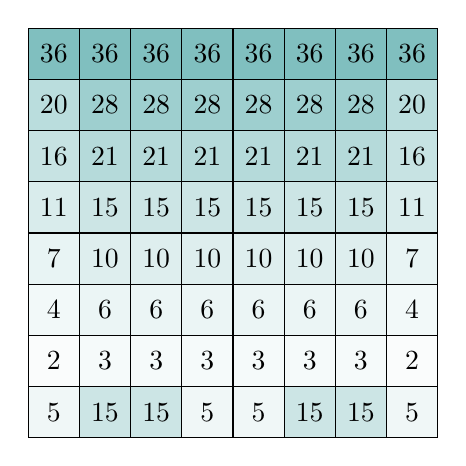
\begin{tikzpicture}[scale=0.65]
        \foreach \row[count=\i] in { {5, 15, 15, 5, 5, 15, 15, 5},     {2, 3, 3, 3, 3, 3, 3, 2},
      {4, 6, 6, 6, 6, 6, 6, 4},         {7, 10, 10, 10, 10, 10, 10, 7},
      {11, 15, 15, 15, 15, 15, 15, 11}, {16, 21, 21, 21, 21, 21, 21, 16},
        {20, 28, 28, 28, 28, 28, 28, 20}, {36, 36, 36, 36, 36, 36, 36, 36}} {
          \foreach \v [count=\j] in \row {
            \pgfmathtruncatemacro{\tmp}{50*\v/36}
            \filldraw[fill=teal!\tmp] (\j,\i) ++ (-0.5,-0.5) rectangle ++(1,1);
            \draw (\j,\i) node {\v};
          }
        }
      \end{tikzpicture}}

  \item Každý bezpečný kameň dostane 50\% bonus oproti hodnote z bodu 2. 
    Kameň je bezpečný, ak má aspoň toľko obrancov, ako útočníkov 
    (t.j. súper nemôže sériou výmen získať kameň). Napr v nasledovnej pozícii sú všetky kamene bezpečné, ale
    ak by bol na ťahu biely a potiahol by \vb{f3-g4}, kameň na pozícii \vb{g4} by už bezpečný nebol. Rovnako,
    keby biely pohol \vb{e4-d5}, kameň na \vb{d5} by nebol bezpečný, lebo by mal dvoch útočníkov (\vb{c6} a \vb{e6})
    a iba jedného obrancu (\vb{c4}); čierny by teda sériou výmen získal o kameň viac. \\


\centerline{
%\tikzset{external/force remake}
\begin{tikzpicture}[scale=0.65]
  \boardBg
  \boardGrid
  \bPs{17,27,37,47,57,67,16,56,66,25,35,45,24,54}
  \wPs{10,20,30,50,60,70,11,21,22,32,52,23,43,53}
\end{tikzpicture}
}
\end{enumerate}


\begin{uloha}
  Doprogramuj do triedy \vb{AlphaBetaPlayer} transpozičné tabuľky a vylepšenú evaluačnú funkciu. Naprogramuj šablónu

  \begin{lstlisting}
template <typename P1, typename P2>
int duel() {
  P1 p1;
  P2 p2;
  ...
}
  \end{lstlisting}

  ktorá si vyrobí dvoch hráčov, zohrá partiu a vráti výsledok.
\end{uloha}

Teraz je čas na experimenty. Je veľa rôznych možností, ako hráča vylepšiť. Na jednej strane je kľúčový parameter počet prehľadaných vrcholov, takže 
sa oplatí jednotlivé časti programu zrýchľovať. Napr. predrátať hešovací kľúč, používať rýchlejšiu špeciálne upravenú hešovaciu tabuľku, rýchlejšie rátať evaluačnú funkciu
a pod. Na druhej strane je snaha viac stromu odrezať, takže napr. lepšie triediť ťahy pri prehľadávaní, prípadne použiť tzv. {\em iterative deepening}, 
\indexItem{Alg}{iterative deepening a podobné vylepšenia}
kde sa postupne
spúšťa prehľadávanie s väčšími a väčšími hĺbkami a na triedenie ťahov sa používajú hodnoty vyrátané v predchádzajúcej iterácii. Ďalej sú to vylepšenia samotného algoritmu: 
dá sa pridať knižnica otvorení (nechať hrať hráča samého proti sebe a pozerať sa, ktoré pozície na začiatku častejšie vedú k výhre; 
tie si potom zapamätať a snažiť sa ich častejšie voliť pri hre), dá sa pridať riešenie koncoviek (buď v situácii, keď už ostáva iba málo kameňov, alebo
keď je niektorý kameň blízko cieľa sa dá buď použiť dynamické programovanie alebo si nejaké patterny predrátať) a pod. 
Takisto sa dá robiť niečo proti tzv. {\em horizon effect}: keďže prehľadávanie ide do fixnej hĺbky, môže sa stať, že originálny algoritmus zastane
uprostred série výmen (napr. biely vyhodí čierneho a má o kameň naviac, ale už sa nezistí, že čierny môže vyhodiť tiež a budú mať rovnako); preto sa zvykne pred skončením
prehľadávania v nulovej hĺbke pokračovať v sérii výmen, kým sa nedostane do ``tichej'' pozície. 

Zopár dobrých nápadov by malo stačiť na to, aby program hral lepšie ako bežný netrénovaný človek. Môžeš používať \vb{duel} na to, aby si si overil, ktoré zmeny 
program zosilnia a ktoré naopak oslabia. 

